\documentclass[12pt]{article}
 
\usepackage[margin=1in]{geometry} 
\usepackage{amsmath,amsthm,amssymb}
\usepackage{hyperref}
\usepackage{graphicx}
\usepackage{xcolor}
\usepackage[many]{tcolorbox}
\tcbuselibrary{listings}
\usepackage{listings}
%jari:
\usepackage{enumitem}

\definecolor{lg}{HTML}{f0f0f0}

\newtcblisting{pycode}{
    colback=lg,
    boxrule=0pt,
    arc=0pt,
    outer arc=0pt,
    top=0pt,
    bottom=0pt,
    colframe=white,
    listing only,
    left=15.5pt,
    enhanced,
    listing options={
        basicstyle=\small\ttfamily,
        keywordstyle=\color{blue},
        language=Python,
        showstringspaces=false,
        tabsize=2,
        numbers=left,
        breaklines=true
    },
    overlay={
        \fill[gray!30]
        ([xshift=-3pt]frame.south west)
        rectangle
        ([xshift=11.5pt]frame.north west);
    }
}

\lstset{
    language=Python,
    basicstyle=\small\ttfamily,
}

 
\begin{document}
 
\title{Exercise 3}
\author{
Jari Mattila - 35260T\\
ELEC-E8125 - Reinforcement Learning}

\maketitle
\section*{Task 1.1}

The training performance plots for each of the tasks (Task 1.1 - fixed and GLIE, Task
1.3 - for both initializations, Task 2 - Lunar Lander).
\newline

NumPy file q\_values.npy, which includes the learned Q-values for Task 1.1 for Cartpole with GLIE, saved when the training has finished (don’t attach the values for contant epsilon)
\newline

NumPy file value\_func.npy, which contains the value function for the same conditions as in the previous point
\newline

\noindent
Source files: qlearning.py, q\_values.npy, value\_func.npy

\section*{Task 1.2}

The heatmap from the end of the training (Task 1.2).
\newline

Plot the heatmap of the value function in terms of x and θ. For plotting, average the
values over $x^{´}$ and $\theta^{}$.

\begin{figure}[h] 
	\centering  % Remember to centre the figure
    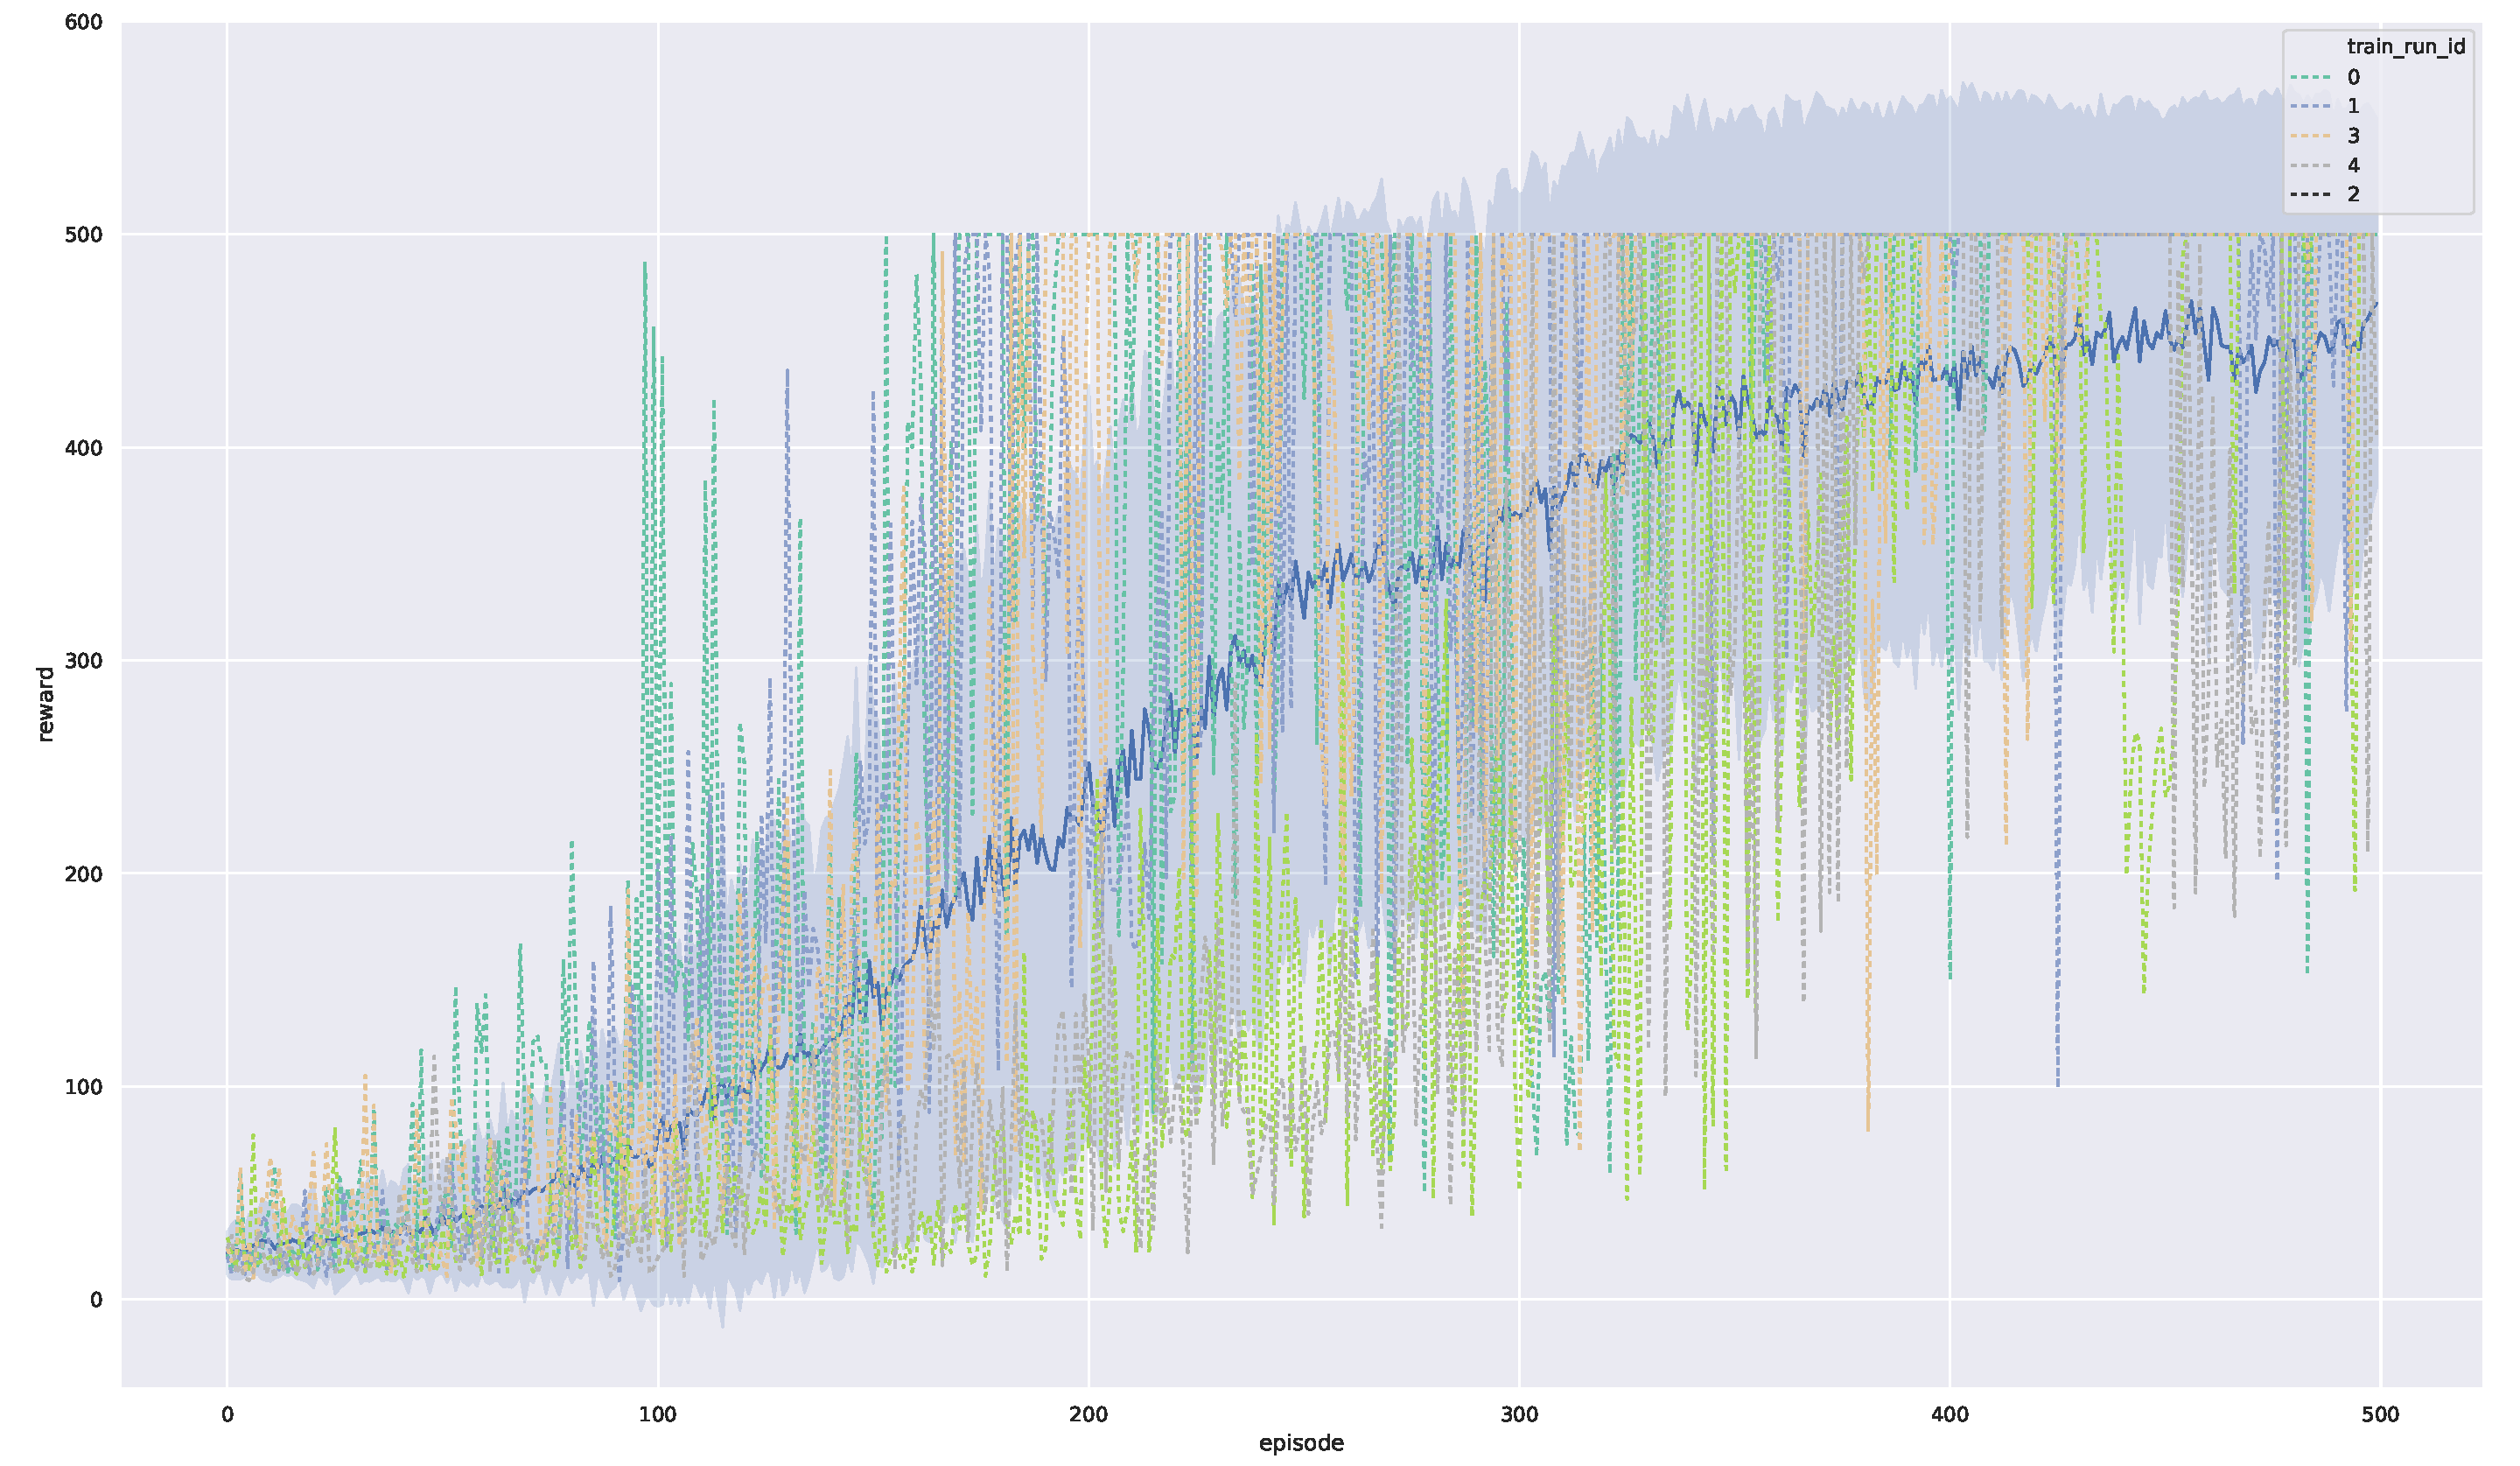
\includegraphics[width=0.9\columnwidth]{img/training.pdf}
	\caption{This is a sample figure.}
	\label{fig:fig1}
\end{figure}

\section*{Question 1}

What do you think the heatmap would have looked like:

%\begin{itemize}
\begin{enumerate}[label=(\alph*)]
    \item before the training?
    \item after a single episode?
    \item halfway through the training?
\end{enumerate}
%\end{itemize}

\noindent
Justify why for all the cases. Attaching the plots is not required.

\section*{Task 1.3}

The training performance plots for each of the tasks (Task 1.1 - fixed and GLIE, Task
1.3 - for both initializations, Task 2 - Lunar Lander).
\newline

\noindent
Source files: qlearning.py

\section*{Question 2}

Based on the results you observed in Task 1.3, answer the following questions:

\section*{Question 2.1}

In which case does the model perform better?

\section*{Question 2.2}

Why is this the case, and how does the initialization of Q values affect exploration?


\section*{Task 2}

The training performance plots for each of the tasks (Task 1.1 - fixed and GLIE, Task
1.3 - for both initializations, Task 2 - Lunar Lander).
\newline

\noindent
Source files: qlearning.py

\section*{Question 3}

Is the lander able to learn any useful behaviour? Why/why not?


\pagebreak


\section{Task 1090}

If you add a figure, you can refer to it using Figure.~\ref*{fig:fig1}.

To cite works, put them in the template.bib file and use~\cite{sutton2018reinforcement}.

\begin{pycode}
for episode_number in range(train_episodes):
    reward_sum, timesteps = 0, 0
    done = False
    # Reset the environment and observe the initial state
    observation = env.reset()

    # Loop until the episode is over
    while not done:
        # Get action from the agent
        action, action_probabilities = agent.get_action(observation)
        previous_observation = observation

        # Perform the action on the environment, get new state and reward
        observation, reward, done, info = env.step(action)

        # Store action's outcome (so that the agent can improve its policy)
        agent.store_outcome(previous_observation, action_probabilities, action, reward)

        # Draw the frame, if desired
        if render:
            env.render()
\end{pycode}

\begin{figure}[h] 
	\centering  % Remember to centre the figure
    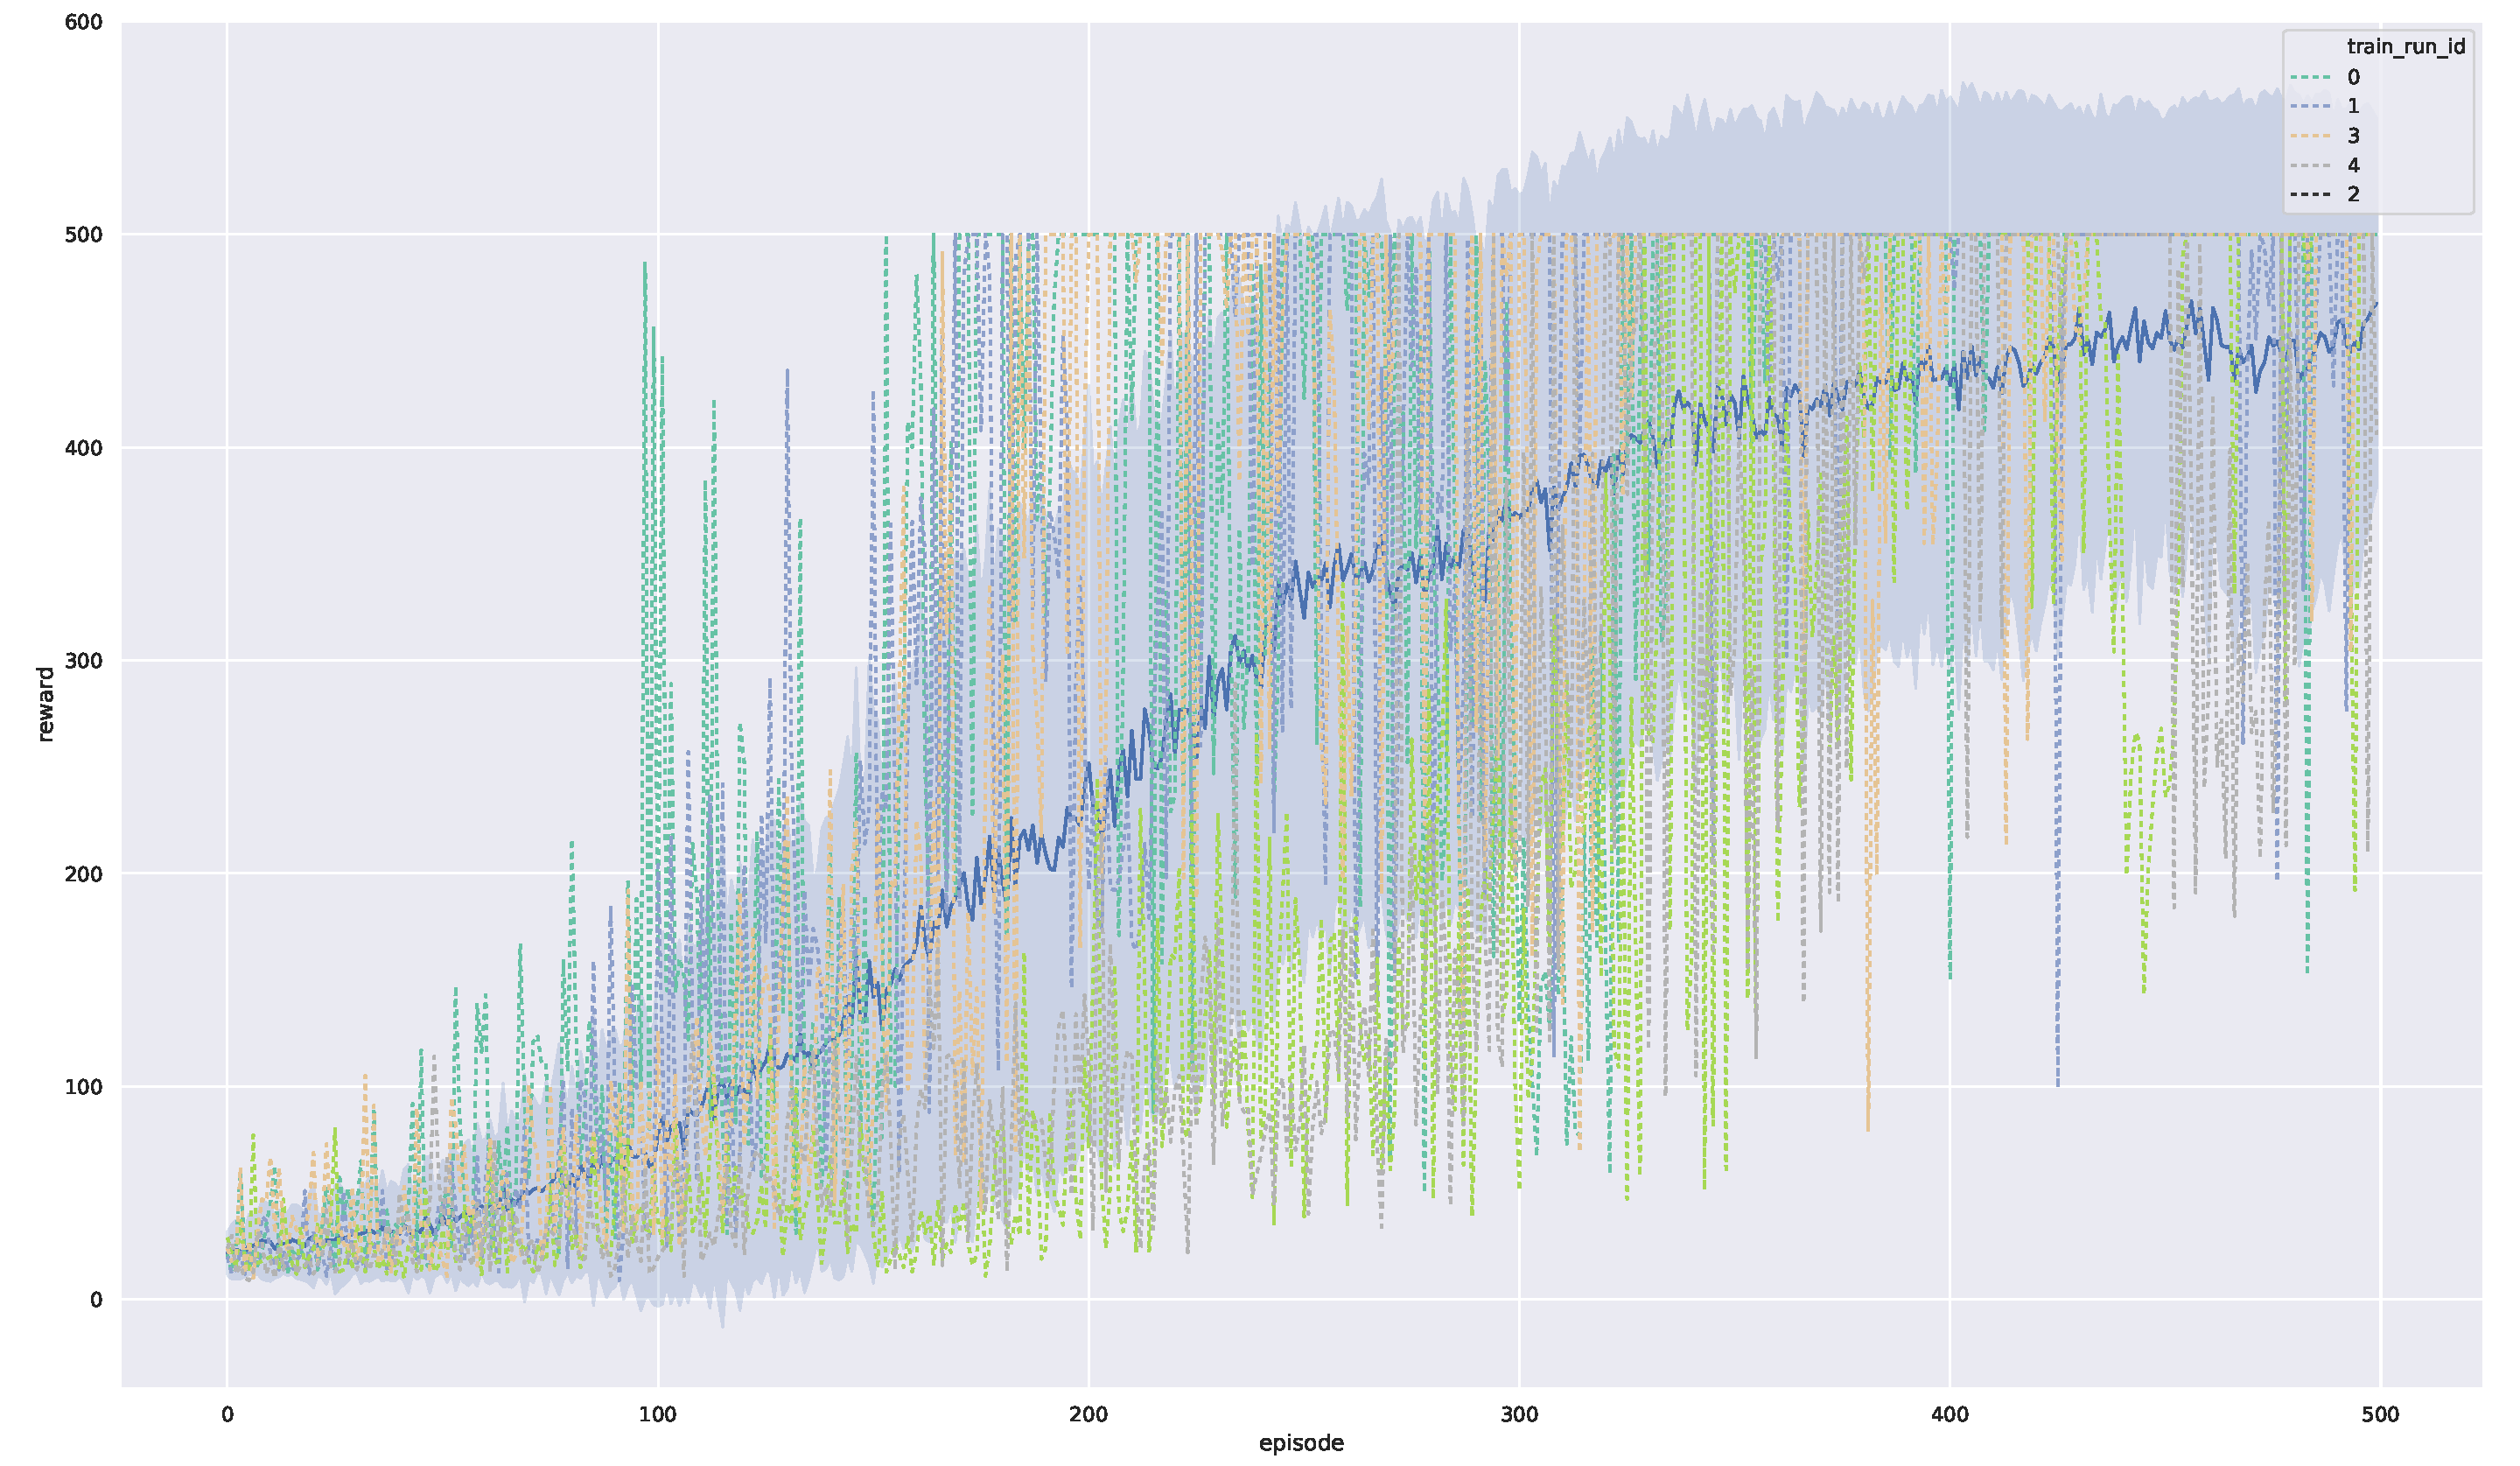
\includegraphics[width=0.9\columnwidth]{img/training.pdf}
	\caption{This is a sample figure.}
	\label{fig:fig1}
\end{figure}

\bibliographystyle{ieeetr}
\bibliography{template}  % Modify template with your bibliography name
\end{document}
